\documentclass[draft,final,openany,oneside]{vutinfth} % Remove option 'final' to obtain debug information.

% Einstellungen für Bilder:
\usepackage{graphicx}
\usepackage{caption}

% FÜR QUELLCODES:
\usepackage{listings}
\usepackage{color,colortbl}
\definecolor{Hellgrau}{gray}{0.92}
% Ende: Quellcode-Settings




\usepackage{lmodern}        % Use an extension of the original Computer Modern font to minimize the use of bitmapped letters.
\usepackage[T1]{fontenc}    % Determines font encoding of the output. Font packages have to be included before this line.
\usepackage[utf8]{inputenc} % Determines encoding of the input. All input files have to use UTF8 encoding.


\usepackage{amsmath}    % Extended typesetting of mathematical expression.
\usepackage{amssymb}    % Provides a multitude of mathematical symbols.
\usepackage{mathtools}  % Further extensions of mathematical typesetting.
\usepackage{microtype}  % Small-scale typographic enhancements.
\usepackage[inline]{enumitem} % User control over the layout of lists (itemize, enumerate, description).
\usepackage{multirow}   % Allows table elements to span several rows.
\usepackage{booktabs}   % Improves the typesetting of tables.
\usepackage{subcaption} % Allows the use of subfigures and enables their referencing.
\usepackage[ruled,linesnumbered,algochapter]{algorithm2e} % Enables the writing of pseudo code.
\usepackage[usenames,dvipsnames,table]{xcolor} % Allows the definition and use of colors. This package has to be included before tikz.
\usepackage{nag}       % Issues warnings when best practices in writing LaTeX documents are violated.
\usepackage{todonotes} % Provides tooltip-like todo notes.
\usepackage{hyperref}  % Enables hyperlinking in the electronic document version. This package has to be included second to last.
\usepackage[acronym,toc]{glossaries} % Enables the generation of glossaries and lists of acronyms. This package has to be included last.

% Define convenience functions to use the author name and the thesis title in the PDF document properties.
\newcommand{\authorname}{Forename Surname} % The author name without titles.
\newcommand{\thesistitle}{Title of the Thesis} % The title of the thesis. The English version should be used, if it exists.

% Set PDF document properties
\hypersetup{
	%pdfpagelayout   = TwoPageRight,           % How the document is shown in PDF viewers (optional).
	linkbordercolor = {Melon},                % The color of the borders of boxes around hyperlinks (optional).
	pdfauthor       = {\authorname},          % The author's name in the document properties (optional).
	pdftitle        = {\thesistitle},         % The document's title in the document properties (optional).
	pdfsubject      = {Subject},              % The document's subject in the document properties (optional).
	pdfkeywords     = {a, list, of, keywords} % The document's keywords in the document properties (optional).
}

\setpnumwidth{2.5em}        % Avoid overfull hboxes in the table of contents (see memoir manual).
\setsecnumdepth{subsection} % Enumerate subsections.

\nonzeroparskip             % Create space between paragraphs (optional).
\setlength{\parindent}{0pt} % Remove paragraph indentation (optional).

\makeindex      % Use an optional index.
\makeglossaries % Use an optional glossary.
%\glstocfalse   % Remove the glossaries from the table of contents.

\enlargethispage{10\baselineskip}

\begin{document}

% Quellcode-Darstellung von Listings
% Doku: https://mirror.ox.ac.uk/sites/ctan.org/macros/latex/contrib/listings/listings.pdf
\lstset{numbers=left, numberstyle=\tiny, stepnumber=2, numbersep=5pt, backgroundcolor=\color{Hellgrau}, columns=[c|l|r]{fullflexible}, breaklines=true, basicstyle=\small\ttfamily}
%% ENDE:Listingseinstellungen


% HIER FINDEN SICH DIE LINKS ZU DEN ALLGEMEINEN KAPITELN
% ab hier: römische Seitenzahlen	
\frontmatter 

\begin{titlepage}
	\thispagestyle{empty} % Unterdrückt die Seitennummerierung auf dieser Seite
	\centering
	\vspace*{1cm}
	{\LARGE \textbf{Meine Titelseite} \par}
	\vspace{1.5cm}
	{\Large Unterüberschrift oder Autor \par}
	\vfill
	{\large Datum \par}
	

\end{titlepage}

\begin{kurzfassung*}
Die App-Programmierung ist ein Schlüsselelement in der digitalen Landschaft, das die Entwicklung von Anwendungen für mobile Geräte wie Smartphones und Tablets umfasst. Mit fundierten Kenntnissen in Programmiersprachen wie Java, Swift und Kotlin sowie in Frameworks wie React Native oder Flutter können Entwickler benutzerfreundliche und leistungsstarke Anwendungen erstellen. Eine gut gestaltete Benutzeroberfläche und eine reibungslose Benutzererfahrung sind entscheidend. Aktuelle Trends umfassen KI-Integration, AR und VR, Blockchain und IoT, die neue Möglichkeiten für innovative und interaktive Apps eröffnen. Die App-Programmierung bietet eine spannende Chance, kreative Ideen in funktionale Anwendungen umzusetzen, die das Leben vieler Menschen bereichern können.
\end{kurzfassung*}
 
\begin{abstract}
App development is a cornerstone of the digital landscape, encompassing the creation of applications for mobile devices such as smartphones and tablets. With proficient knowledge in programming languages like Java, Swift, and Kotlin, as well as frameworks like React Native or Flutter, developers can craft user-friendly and powerful applications. A well-designed user interface and smooth user experience are crucial. Current trends include AI integration, AR and VR, Blockchain, and IoT, which offer new avenues for innovative and interactive apps. App development presents an exciting opportunity to translate creative ideas into functional applications that can enrich the lives of many.
\end{abstract} 
\begin{eides}
Ich erkläre an Eides statt, dass ich die vorliegende Diplomarbeit selbstständig und ohne fremde Hilfe verfasst, keine anderen als die angegebenen
Quellen und Hilfsmittel benutzt und die den benutzten Quellen wörtlich und inhaltlich entnommenen Stellen als solche erkenntlich gemacht habe.
	
\vspace{20pt}	
\begin{flushright}
		St. Pölten, 31.Jänner 2025
\end{flushright}
	
\end{eides} 
\begin{danksagung}
Mein herzlicher Dank gilt meinem Technologiemangement-Lehrer für seine  Unterstützung bei der Erstellung der \LaTeX-Vorlage. Außerdem bedanke ich mich bei meinen Eltern und meiner Tante für das Korrekturlesen.
\end{danksagung} 

% Sprache wählen: english or naustrian.
\selectlanguage{naustrian}

% Inhaltsverzeichnis
\tableofcontents 

% Nummerierung ändern auf arabische Ziffern
\mainmatter


% AB HIER STARTEN DIE INHALTLICHEN KAPITEL
\chapter{Einleitung}
In der heutigen digitalen Ära spielt die Entwicklung von Anwendungssoftware eine immer wichtigere Rolle, insbesondere im Kontext der zunehmenden Digitalisierung verschiedener Aspekte des täglichen Lebens.


\section{Bestehende Software}
Apps können durch die Verwendung verschiedener Programmiersprachen wie Java, Kotlin für Android oder Swift für iOS entwickelt werden. Die Entwicklungsumgebung bietet Werkzeuge wie Android Studio für Android oder Xcode für iOS, die Entwicklern helfen, Benutzeroberflächen zu gestalten, Funktionalitäten zu implementieren und mit APIs zu interagieren. Anschließend wird die App auf einem Emulator oder einem physischen Gerät getestet und schließlich in den jeweiligen App Stores veröffentlicht. Selbst Alan Turing (vgl.~\cite{Turing1936}) konnte das nicht ahnen.


\subsection{Android}
Android ist ein Betriebssystem für mobile Geräte, das von Google entwickelt wird (siehe \cite{android}). Es basiert auf dem Linux-Kernel und bietet eine offene Plattform für Entwickler. Android ermöglicht die Entwicklung vielfältiger Anwendungen, von Spielen über Produktivitäts-Apps bis hin zu sozialen Medien. Der Google Play Store bietet eine riesige Auswahl an Apps für Android-Geräte.

 

\chapter{Theorie}
Auch hier stehen wieder ein paar Zeilen Text.
	
	
\section{Über Anroid Studio}
Apps können durch die Verwendung verschiedener Programmiersprachen wie Java, Kotlin für Android oder Swift für iOS entwickelt werden. Die Entwicklungsumgebung bietet Werkzeuge wie Android Studio für Android oder Xcode für iOS, die Entwicklern helfen, Benutzeroberflächen zu gestalten, Funktionalitäten zu implementieren und mit APIs zu interagieren. Anschließend wird die App auf einem Emulator oder einem physischen Gerät getestet und schließlich in den jeweiligen App Stores veröffentlicht.

\section{Aufzählungen}
Auch bei Aufzählungen sollte man entsprechende Befehle verwenden.
\begin{itemize}
	\item \textbf{Lehrer:} Das ist jetzt nur ein Demotext, der über eine Zeile geht. Hier wird ersichtlich, dass man sich nicht um Abstände etc. kümmern muss.
	\item Schüler: Bei diesem Aufzählungspunkt ist das erste Worte nun nicht fett geschrieben.
	\item Räume
\end{itemize}

Natürlich kann man auch nummerierte Aufzählungen einfügen:
\begin{enumerate}
	\item TMAN
	\item HAK
	\item St. Pölten
\end{enumerate} 

\chapter{Programmierung der App}
% Codedarstellung - Hinweise
% in 00_Einstellungen wird das Paket eingebunden
% in diplomarbeit.tex gibt es weitere Details dazu

\section{Struktur}
Im folgenden Abschnitt wird die Generelle Klassenstruktur vorgestellt

% Code-BEGINN
\begin{lstlisting}	
	class
	{
	 public:
		// Oefentliche Methoden
	        void Initialize(); 
		void Update(); 
		void Draw(); 
 	 private: 
		// Private Methoden
	 public: 
		// Oeffentliche Variablen
	 private:
		// Private Variablen
	};
\end{lstlisting}
\captionof{lstlisting}{Klassenstruktur}
% Code-ENDE

% Code-BEGINN
\section{Schreibstil}
Das gesamte Programm wurde mit einem einheitlichen Stil geschrieben, dieser wird in diesem Abschnitt vorgestellt. 

Methoden beginnen immer mit einem Großbuchstaben, so werden diese klar von Variabeln getrennt.

% Code-BEGINN
\begin{lstlisting}	
	class
	{
	 public:
		void Beispielsmethode(); 
	};
\end{lstlisting}
\captionof{lstlisting}{Methoden}
% Code-ENDE

Variablen welche member einer Klasse sind werden mit einem preafix gekennzeichnet und kleingeschrieben

% Code-BEGINN
\begin{lstlisting}
	class
	{
		// Methoden
		...
	 public: 
		// Oeffentliche Variablen werden mit dem Praefix p_ makiert
	 private:
		// Private Variablen werden mit dem Praefix m_ makiert
	};
\end{lstlisting}
\captionof{lstlisting}{membervariabeln}
% Code-ENDE

Lokale Variabeln zu gänze kleingeschrieben und erhalten keinen Praefix. 

% Code-BEGINN
\begin{lstlisting}
	class
	{
	 public:
		void Beispielsmethode()
		{
			int beispielsvariabel; 
		}
		...
		// Membervariabeln
	};
\end{lstlisting}
\captionof{lstlisting}{lokale variabeln}
% Code-ENDE

Bei Parametern wird der erste Buchstabe großgeschrieben, dadurch können Parameter von Member- und Lokalvariabeln unterschieden. 
 
% Code-BEGINN
\begin{lstlisting}
	class
	{
		public:
		void Beispielsmethode(int Beispielsparameter)
		{
			int beispielsvariabel = Beispielsparameter; 
		}
		...
		// Membervariabeln
	};
\end{lstlisting}
\captionof{lstlisting}{Parameter}
% Code-ENDE



% Noch nicht Fomratier  oder in richtiger Reinfolge
\section{Generieren der Karte}

Jedes Spiel braucht eine Karte, in diesem Abschnitt werden wir uns Schrittweise die Implementierung der Map Klasse anschauen. 
% Code-BEGINN

\begin{lstlisting}
class Map
{
public:
	Map()
	{}
	
	void Initialize();
	void Generate();
	void Draw();
	... 
};
\end{lstlisting}
\captionof{lstlisting}{Map}
% Code-ENDE

Die Methode "Initialize" hat den Zweck member Variablen einen Wert zuzuweisen und gegenbenfalls in der Klasse enthaltene Objekte zu Initalisieren.
\begin{lstlisting}
	...
	void Initialize();
	...
\end{lstlisting}

Die Idee ist es die Karte als 2-Demensionales Liste aus "Tiles"  darzustellen, vorab definieren wir also die Größe Karte, sowie die Größe der "Tiles". 
\begin{lstlisting}
	...
	void Initialize(const sf::Vector2u& tilesize, const int& width, const int& height);
	...
\end{lstlisting}

Diese Werte sollen in der Klasse abgespeichert werden. Daher definieren wie nun die drei Member "tilesize", "width", und "height". 
\begin{lstlisting}
	...
 	private: 
 		sf::Vector2u m_tilesize; 
 		int m_width; 
 		int m_height; 
	...
\end{lstlisting}

Anschließend weisen wir den Membern den jewiligen Parametern zu. 

\begin{lstlisting}
	...
	void Initialize(const sf::Vector2u& tilesize, const int& width, const int& height)
	{
		m_tileSize = tilesize;
		m_width = width; 
		m_height = height; 
	}
	...
\end{lstlisting}

\captionof{lstlisting}{Map::Initialize()}

Die Methode ist vorerst fertiggestellt, nächster Schritt ist nun die Generierung. Wie schon erwähnt ist die Idee, die Karte als 2-Demensionale Liste bestehend aus "Tiles" darzustellen. Ähnlich wie das auch andere Spielen machen. (Beispiel Anführen) Die einzelnen Tiles sollen Informationen über Textur, Position und deren ID beeinhalten. Hierfür verwenden wir den Datentyp "Struct". Structs unterscheiden sich in c++ nicht wesentlich von Klassen, jedoch werden wir aus Stilgründen den Typ Struct verwenden. Wichtig: Structs sollen jediglich informationen beeinhalten und üben sonst keine Funktion aus. 



\begin{lstlisting}
	struct Tile
	{
		...
		unsigned int tile_ID;
		sf::Vector2f tile_position;
		
		sf::IntRect* tile_texRect;
		sf::Sprite   tile_sprite;
		
	};
\end{lstlisting}
	

Der Konstruktor wird definiert, wir erfassen die ID, die Position und die Textur. 
\begin{lstlisting}
	...
	Tile(const unsigned int& ID, sf::IntRect* TextureRectangle, const sf::Sprite &Sprite, const sf::Vector2f& TilePosition)
	...
\end{lstlisting}

Die die Member werden mit den Parametern initialsiert 
\begin{lstlisting}
	...
	: tile_ID(ID), tile_texRect(TextureRectangle), tile_sprite(Sprite), tile_position(TilePosition)
	...
\end{lstlisting}

Der Textur wird die Position und Texture Rectangle zugewiesen. 
\begin{lstlisting}
	...
	{
		tile_sprite.setPosition(tile_position);
		tile_sprite.setTextureRect(*tile_texRect); 
	}
	...
\end{lstlisting}

Alle Teile zusammen ergeben einen Funktionierenden Datentyp in dem wir alle notwendigen Information Speichern. 
\begin{lstlisting}
	struct Tile
	{
		Tile(const unsigned int& ID, sf::IntRect* TextureRectangle, const sf::Sprite &Sprite, const sf::Vector2f& TilePosition)
		: tile_ID(ID), tile_texRect(TextureRectangle), tile_sprite(Sprite), tile_position(TilePosition) 
		{
			tile_sprite.setPosition(tile_position);
			tile_sprite.setTextureRect(*tile_texRect); 
		}
		...
	};
\end{lstlisting}

Doch noch ein Schritt fehlt um mit der Generierung zu Starten. Da die Karte in der Klasse abgespeichert werden soll fügen wir den entsprechenden Member hinzu. 
Hiefür verwenden wir den Typ std::vector. Dieser fungiert als herkömmliche liste, die aber nicht statisch initalisiert werden muss wie es beispielsweise bei 
Tile arr[]; der Fall wäre. Später sollen andere Klassen noch auf die Karte zugreifen also schreiben wir sie als public. 
\begin{lstlisting}
	...
	std::vector<std::vector<Tile>> p_tileMap;
	...
\end{lstlisting}

\captionof{lstlisting}{Tile}

Nach dem alle vorbereitungen getroffen worden sind, können wir mit der Generierung beginnen. 

\begin{lstlisting}
	...
	void Generate();
	...
\end{lstlisting}

Zunächst wollen wir p\_tilemap mit Tiles füllen. Dafür iterieren wir entlang der x-achse und erstellen einen std::vector den wir mit den noch leeren Tiles füllen. Anchließend wird der gefüllte std::vector an p\_tilemap angefügt.

\begin{lstlisting}
void Generate()
{
	for (int i = 0; i < m_width; i++)
	{
		std::vector<Tile> tileMap_row;
		
		for (int j = 0; j < m_height; j++)
		{
			
			tileMap_row.push_back(tile);
		}
		
		p_tileMap.push_back(tileMap_row);
	}
}
\end{lstlisting}
An dieser Stelle verwenden wir Prozedurale Generation - Diese ist zu diesem Zeitpunkt nicht implementiert oder Erklärt. Daher machen wir uns eine Mentale Notiz und 
kommen später wieder zurück. Die grundsätzliche Idee ist es eine 2-Demensionale Liste mit Semi-Zufälligen Werten zu füllen. Jeder dieser Werte stellt ein Bestimmtes Biom da. Demnach laden wir die textur welche dem Biom entspricht. Vorerst schreiben wir also: 
\begin{lstlisting}
...
int biome = // Das Biom an der stelle [i][j]
...
\end{lstlisting}

Wir verwenden das Biom um die richtige Textur, sowie die richtige Position zu finden. 
\begin{lstlisting}
...
sf::IntRect texRect(m_tileSize.x * biome, 
		           m_tileSize.y * biome, 
			   m_tileSize.x, m_tileSize.y);
sf::Vector2f tilePos(m_tileSize.x * i, m_tileSize.y * j);
...
\end{lstlisting}

Anschließend verwenden wir den Konstrukter des Tile-Struct um dem Tile die Daten zuzuweisen. 

\begin{lstlisting}
	...
	Tile tile(index, biome, &texRect, m_tilesprite, tilePos);
	...
\end{lstlisting}

Die vollständige Methode: 

\begin{lstlisting}
void Generate()
{
 for (int i = 0; i < m_width; i++)
 {
  std::vector<Tile> tileMap_row;
  for (int j = 0; j < m_height; j++)
  {
   int biome = // Das Biom an der stelle index
			
   sf::IntRect texRect(m_tileSize.x * biome, 
   			      m_tileSize.y * biome, 
   			      m_tileSize.x, m_tileSize.y);
   					   
   sf::Vector2f tilePos(m_tileSize.x * i, m_tileSize.y * j);
			
   Tile tile(index, biome, &texRect, m_tilesprite, tilePos);
			
   tileMap_row.push_back(tile);
  }
		
  p_tileMap.push_back(tileMap_row);
 }
}
\end{lstlisting}

\captionof{lstlisting}{Map::Generate()}

Nachdem wir Initalize() und Generate() bereits erstellt haben, fehlt uns nur noch Draw(). 

\begin{lstlisting}
	...
	void Draw();
	...
\end{lstlisting}

Vorerst hat die Methode nur die Aufgabe alle Texturen der Tiles zu zeichnen. Das problem ist hierbei aber das wir gleich die Ganze Map rendern, das wiederrum führt zu problemen mit der Performance. Es sollte also nur ein Teil bzw. "Chunk" der Map gerendert werden. 

\begin{lstlisting}
	void Draw(sf::RenderWindow& Window)
	{
		for(auto& i : p_tilemap){
			for(auto& j : i){
				window.draw(j.tile_sprite); 
			}
		}	
	}
\end{lstlisting}

Die Map-Klasse ist Fertig. (Vorerst)
Auf der TO-DO-List: Prozedurale Generation mit Perlin Noise und Chunk rendering

\captionof{lstlisting}{Map::Draw()}

\newpage
\section{Der Spieler}

Erste uebersicht der Klasse: 
\begin{lstlisting}
class Player
{
 public:
	void Initalize();
	void Update();
	void Draw();
	
 private:
	void MovePlayer();
};
\end{lstlisting}

Wir beginnen mit der Methode Initlize(), zweck der Methode sollte zu diesem Punkt schon klar sein. Wir stellen uns also die Frage welche Daten die Klasse beeinhalten Soll. 
fuer dieses Projekt werden wir folgende verwenden: Geschwindigkeit, Lebenspunkte, Position, die Hitbox* und die Textur. als public schreiben wir die Hitbox, Position und Lebenspunkte. Der Rest wird als privat geschrieben. 

\begin{lstlisting}
	...
	void Initalize();
	...
\end{lstlisting}

\begin{lstlisting}
	...
public:
	sf::RectangleShape p_hitbox;
	int				   p_health;
private:
	sf::Sprite		   m_sprite;
	sf::Vector2f	   m_position;
	float			   m_speed;
	int movementIndicator = 0; // wird spaeter erklaert 
	
\end{lstlisting}

Nun fuegen wir die notwendigen hinzu und initalisieren die Member. 

\begin{lstlisting}
...
void Initalize(Textureholder& Textures, const float& Speed, const int& Health, const sf::Vector2f& Position);
...
\end{lstlisting}

Das für dieses Projekt verwendete Spieler-Sprite hat eine größe von 64x64 daher setzten wir in sf::IntRect die breite sowie die höhe auf 64 pixel. Die hitbox soll der Spritegröße entsprechen und bekommt daher den selben wert zugewiesen. Wir verwenden den Textureholder* um auf die Spieler Textur zuzugreifen. 

\begin{lstlisting}
	...
	m_sprite.setTexture(Textures.Get(Textures::ID::Player));
	m_sprite.setTextureRect(sf::IntRect(0, 0, 64, 64));
	m_sprite.setPosition(Position);
	
	p_hitbox.setSize(sf::Vector2f(64, 64));
	...
\end{lstlisting}

Die Update Methode der Spieler klasse soll die Spielerbewegungen festhalten, daher verändern wir die Position um die Geschwindigkeit * Deltatime gleichzeitg verschieben wir den Ausschnitt der textur (TextureRectangle). Fue diesen Zweck definieren wir die Makros* UPWARDS, DOWNWARDS, LEFTWARDS und RIGHTWARDS. die Werte stellen die Position in der jeweiligen Sprites innerhalb der Textur da. Um festzustellen ob die Spielerposition sich mit einem Hinderniss überschneidet übergeben wir die Map-Klasse an die Methode. Zusätzlich passen wir die Hitbox an die positon des Spielers an. 


\begin{lstlisting}
	...
	#define FORWARD 0
	#define LEFTWARD 1
	#define BACKWARD 2
	#define RIGHTWARD 3
	...
\end{lstlisting}

\begin{lstlisting}
	...
	void Update(const float& Deltatime, MapGenerator &Map)
	{
		MovePlayer(Deltatime, Map);
		p_hitbox.setPosition(m_position);
	}
	...
\end{lstlisting}

Definieren wir die MovePlayer Methode. 
\begin{lstlisting}
	...
	private: 
	 void MovePlayer(const float &Deltatime, MapGenerator &Map); 
	...
\end{lstlisting}

Fuer jede der Richtung verwenden die von SFML bereitsgestellte Methode " sf::KeyBoard::isKeyPressed ". Diese registriert eingaben die über die Tastatur getaetigt werden. 

\begin{lstlisting}
	...
	if (sf::Keyboard::isKeyPressed(sf::Keyboard::W))
	...
\end{lstlisting}

wir legen die neue position fest. Da der Spieler in richtung oben laufen soll multiplplizieren wir die änderung an der y-achse mit -1. Das funktioniert weil der 
punkt (0,0) Oben-Links befindet. (Quelle)  

\begin{lstlisting}
	...
	sf::Vector2f newposition = m_position + sf::Vector2f(0, -1) * m_speed * dt; 
	...
\end{lstlisting}

An dieser stelle ist anzumerken das es wohl bessere wege gaebe um das problem zu lösen. Da der Userinput bei jeder iteration der Update methode abgefragt wird, kommt es zu mehreren hunderten abfragen pro sekunde. Da das sich nicht mit der Anfordung ein visuell stimulierendes Spiel zu programmieren deckt, verhindern wir dies in dem wir eine 
Membervariabel deklarieren welche bei jeder Iteration mitlaeuft. Die Werte 9 und 5 sind hier trivial.  
\newline 
Zuletzt weisen wir den Member m\_position die neue position zu.  
\begin{lstlisting}
	...
	m_sprite.setPosition(newposition);

	m_sprite.setTextureRect(sf::IntRect((movementIndicator / 5) * SPRITEUNIT, FORWARD, SPRITEUNIT, SPRITEUNIT));
	movementIndicator++;
	if (movementIndicator / MOVEMENT == 9) {
		movementIndicator = 0;
	}
	

	m_position = m_sprite.getPosition();
}
...
\end{lstlisting}

Da wir verhindert müssen das der Spieler mit hindernissen kollidert ueberpruefen wir ob die Spielerpostion auf der Tilemap bereits belegt ist. Dauer definieren wir die
methode YouShallPass.

\begin{lstlisting}
	...
	bool YouShallPass(const sf::Vector2f& reisepass, MapGenerator &map) {
		int x = reisepass.x / map.GetTileSize().x, y = reisepass.y / map.GetTileSize().y; 
		if (map.p_tileMap[x][y].occupied != true) {
			return true; 
		}
		return false; 
	}
	...
\end{lstlisting}

Da mit der jetzigen programmierung der Spieler daran gehindert wäre durch gegner durchzulaufen schreiben wir uns noch die Hilfsfunktion "IsEnemy" diese überprüft ob sich die positon mit einem gegner überschneiden würde. Wir verwenden wir den Member des Tile-Structs welche wir im Kapitel 3.3 bereits kennengelernt haben, occupationID. 

\begin{lstlisting}
	...
	bool IsEnemy(MapGenerator& map, const int& x, const int& y) {
		Textures::ID type = map.p_tileMap[x][y].occupationID; 
		switch (type)
		{
			case Textures::ID::Zombie:
			return true; 
		}
		
		return false; 
	}
	...
\end{lstlisting}

Anschließend fuegen wir der Abfrage in der YouShallPass Methode noch die IsEnemy option hinzu.

\begin{lstlisting}
	...
    if (map.p_tileMap[x][y].occupied != true || IsEnemy(map, x,y)) 
	...
\end{lstlisting}

Der Code-Block wird zusättzlich noch für die fälle S, A und D bzw. (0, 1), (-1, 0), (1, 0) wiederhohlt.  

\begin{lstlisting}
	...
	void MovePlayer(const float& dt, MapGenerator& map)
	{
		if (sf::Keyboard::isKeyPressed(sf::Keyboard::W)) {
			sf::Vector2f newposition = m_position + sf::Vector2f(0, -1) * m_speed * dt; 
			
			if (YouShallPass(newposition, map)) {
				m_sprite.setPosition(newposition);
				m_sprite.setTextureRect(sf::IntRect((movementIndicator / MOVEMENT) * SPRITEUNIT, FORWARD, SPRITEUNIT, SPRITEUNIT));
				movementIndicator++;
				if (movementIndicator / MOVEMENT == 9) {
					movementIndicator = 0;
				}
			}
			
		}
		...
		
		m_position = m_sprite.getPosition();
	}
	...
\end{lstlisting}



\newpage
\section{Perlin Noise}
$\sum$

\begin{lstlisting}
DOOOOOD
\end{lstlisting}








 

\chapter{Prozessmanagement}
Da stehen wieder ein paar Zeilen. Dieser Text verweist sogar auf das Bild \ref{fig:BildPSP}, welches einen Projektstrukturplan zeigt. Man kann mit \LaTeX auch auf eine Subsection verweisen, wie etwa auf die folgende mit der Nr. \ref{subsec:PSP} verweisen.

\section{Projektstrukturplan}
\label{subsec:PSP}

\begin{figure}
	\centering
	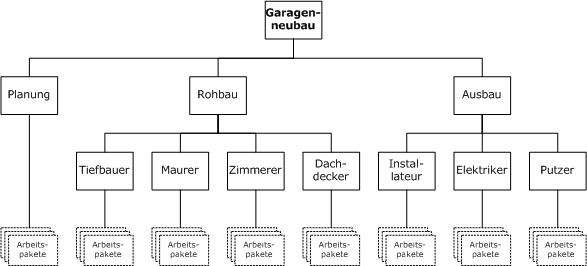
\includegraphics{Bilder/PSP.jpg}
	\caption{Demo-Projektstrukturplan}
	\label{fig:BildPSP}
\end{figure}

\section{Arbeitspakete}
\section{Projektwürdigkeitsanalyse}
\section{Projektdurchführbarkeitsanalyse}
\section{Meilensteinplan}
\section{Tätigkeitsliste - PersonA}

Tabellen einfügen ist in \LaTeX etwas schwieriger. Für das Grundgerüst bieten sich Online-Editoren wie etwa https://latex-editor.pages.dev/table/ an. Dabei ist dann der Tabular-Block zu kopieren.


\begin{table}
\caption{Demotabelle}
\begin{center}
	
\begin{tabular}{ |c|c|c| }
	\hline
	Tätigkeit & Datum & Zeitdauer \\
	\hline
	A         & B     & C         \\
	\hline
	D         & E     & F         \\
	\hline
		D         & E     & F         \\
	\hline
		D         & E     & F         \\
	\hline
		D         & E     & F         \\
	\hline
		D         & E     & F         \\
	\hline
		D         & E     & F         \\
	\hline
		D         & E     & F         \\
	\hline
		D         & E     & F         \\
	\hline
		D         & E     & F         \\
	\hline
\end{tabular}

\end{center}
\end{table} 


\backmatter



% =============================
% Abbildungsverzeichnis
\listoffigures % Starred version, i.e., \listoffigures*, removes the toc entry.
\newpage
% =============================
% Tabellenverzeichnis.
%\cleardoublepage % Start list of tables on the next empty right hand page.
\listoftables % Starred version, i.e., \listoftables*, removes the toc entry.
\newpage


\lstlistoflistings
% =============================

% Optional: Algorithmus-Liste
%\listofalgorithms
%\addcontentsline{toc}{chapter}{List of Algorithms}
% =============================
% Optional: Stichwortverzeichnis
%\printindex
% =============================
% Add a glossary.
% \printglossaries
% =============================
% INHALTSVERZEICHNIS INKL. ZITIERSTIL.
\bibliographystyle{alpha}
\bibliography{intro}
% =============================


\end{document}